\documentclass[paper=a4, fontsize=11pt]{scrartcl} 

\usepackage[T1]{fontenc} 
\usepackage[english]{babel}
\usepackage{amsmath,amsfonts,amsthm}

\usepackage{lipsum}

\usepackage{graphicx}
\usepackage{float}
  \floatplacement{figure}{H}
  \floatplacement{table}{H}
  
\usepackage{sectsty} 
\allsectionsfont{\centering \normalfont\scshape} 

\usepackage{fancyhdr} % Custom headers and footers
\pagestyle{fancyplain} % Makes all pages in the document conform to the custom headers and footers
\fancyhead{} % No page header - if you want one, create it in the same way as the footers below
\fancyfoot[L]{} % Empty left footer
\fancyfoot[C]{} % Empty center footer
\fancyfoot[R]{\thepage} % Page numbering for right footer
\renewcommand{\headrulewidth}{0pt} % Remove header underlines
\renewcommand{\footrulewidth}{0pt} % Remove footer underlines
\setlength{\headheight}{13.6pt} % Customize the height of the header

\usepackage[labelformat=empty]{caption}
\usepackage{color}
\usepackage{listings}
\lstset{ %
language=bash,                % choose the language of the code
basicstyle=\footnotesize,       % the size of the fonts that are used for the code
numbers=left,                   % where to put the line-numbers
numberstyle=\footnotesize,      % the size of the fonts that are used for the line-numbers
stepnumber=1,                   % the step between two line-numbers. If it is 1 each line will be numbered
numbersep=5pt,                  % how far the line-numbers are from the code
backgroundcolor=\color{white},  % choose the background color. You must add \usepackage{color}
showspaces=false,               % show spaces adding particular underscores
showstringspaces=false,         % underline spaces within strings
showtabs=false,                 % show tabs within strings adding particular underscores
frame=single,           % adds a frame around the code
tabsize=2,          % sets default tabsize to 2 spaces
captionpos=b,           % sets the caption-position to bottom
breaklines=true,        % sets automatic line breaking
breakatwhitespace=false,    % sets if automatic breaks should only happen at whitespace
escapeinside={\%*}{*)}          % if you want to add a comment within your code
}
\usepackage{hyperref}


\numberwithin{equation}{section} % Number equations within sections (i.e. 1.1, 1.2, 2.1, 2.2 instead of 1, 2, 3, 4)
\numberwithin{figure}{section} % Number figures within sections (i.e. 1.1, 1.2, 2.1, 2.2 instead of 1, 2, 3, 4)
\numberwithin{table}{section} % Number tables within sections (i.e. 1.1, 1.2, 2.1, 2.2 instead of 1, 2, 3, 4)

\setlength\parindent{0pt} % Removes all indentation from paragraphs - comment this line for an assignment with lots of text

%----------------------------------------------------------------------------------------
%	TITLE SECTION
%----------------------------------------------------------------------------------------

\newcommand{\horrule}[1]{\rule{\linewidth}{#1}} % Create horizontal rule command with 1 argument of height

\title{	
\normalfont \normalsize 
\textsc{Computational Science - ITB} \\ [25pt] % Your university, school and/or department name(s)
\horrule{0.5pt} \\[0.4cm] % Thin top horizontal rule
\small  Pengenalan Sains Komputasi - RandomWalk\\ % The assignment title
%\horrule{2pt} \\[0.5cm] % Thick bottom horizontal rule
}

\author{\small{Ridlo W. Wibowo || 20912009}} % Your name

\date{\normalsize\today} % Today's date or a custom date

\begin{document}

\maketitle % Print the title

\large \textbf{Problem 1.}\\
A hiker without a compass trying to find the way in the dark can step in any of eight directions (N, NE, E, SE, E, SW, W, NW) each step. Studies show that people tend to veer to the right under such circumstances. Initially, the hiker is facing north. Suppose at each step probabilities of going in the indicated directions are as follows: N\---19\%, NE\---24\%, E\---17\%, SE\---10\%, S\---2\%, SW\---3\%, W\---10\%, NW\---15\%. Develop a simulation to trace a path of hiker, and run the simulation a number of times. Describe the results. (Note that other than at the initial step, this simulation simplifies the problem by ignoring the direction in which the hiker faces.)\\

\large \textbf{Problem 1.}\\
Perform a simulation of Brownian Motion of a pollen grain suspended in a liquid by generating a three dimensional random walk. Using documentation for your computational tool, investigate how to plot three dimensional graphics and lines, and create a 3D graphic of the walk.


\vspace{2cm}
\large \textbf{Documentation.}\\
\textit{\textbf{A hiker without a compass}}\\
Permasalahan ini menganggap bahwa probabilitas untuk \textit{hiker} melangkah ditentukan oleh probabilitas di atas. Probabilitas tersebut hanya bergantung kepada arah angin (penyederhanaan) tidak berdasarkan kemana \textit{hiker} menghadap (lebih alami). Untuk itu dibuat simulasi \textit{randomwalk} dimana langkah \textit{hiker} dianggap tetap kemanapun ia berjalan dan probabilitas ke arah mana ditentukan dengan cara \textit{roullete} menggunakan distribusi kumulatif sesuai persoalan yang diberikan. Tiap pengambilan langkah dilakukan dengan melihat angka random yang dicocokkan dengan \textit{roulette} tersebut. \\

Langkah dan arah tersebut ditentukan dengan menggunakan sudut (koordinat polar), sehingga perlu konversi ke koordinat kartesian setiap waktu, walaupun sebenarnya dalam kasus sederhana ini langkah yang diambil pasti hanya berupa konstanta (langkah \textit{hiker} dianggap tetap). Hal ini membuat program ini tidak terlalu efektif, namun dengan cara ini lebih mudah untuk membayangkan dan memahami permasalahan.\\

Program dalam bahasa C++ diberikan di bawah ini (berserta fungsi plot dan animasi menggunakan \textit{gnuplot}):
\lstset{frameround=fttt}
\begin{lstlisting}
/*********************************************/
/* hiker.cpp                                 */
/* Copyleft (c) 2012. Ridlo W. Wibowo        */
/*********************************************/
#include <iostream>
#include <stdio.h>
#include <stdlib.h>
#include <math.h>
#include <time.h>
#include <fstream>
#define _USE_MATH_DEFINES
using namespace std;

double unirand(){ return (double)rand()/(double)RAND_MAX;}

/************************************************************/
/* N-19%, NE-24%, E-17%, SE-10%, S-2%, SW-3%, W-10%, NW-15% */
/* cumulative                                               */
double randtheta(){
       double p = unirand();
       if (p < 0.19){ return 0.5*M_PI;} // N
       else if (p < 0.43){ return 0.25*M_PI;} // NE
       else if (p < 0.60){ return 0.0;} // E
       else if (p < 0.70){ return 1.75*M_PI;} // SE 
       else if (p < 0.72){ return 1.5*M_PI;} // S
       else if (p < 0.75){ return 1.25*M_PI;} // SW
       else if (p < 0.85){ return M_PI;} // W
       else{ return 0.75*M_PI;} // NW
}

void plot(double Rmax);
void animate(int n, double Rmax);

int main(){
    double step=1.0; // hiker's step is constant: 1 m
    double theta=0.0;
    double Rmax=30;
    double x=0., y=0., dx=0., dy=0., r=0.; // initial at 0,0
    int n = 0;

    ofstream out("hiker-out.txt");
    srand(time(NULL));
    do{
        theta = randtheta();
        dx = step*cos(theta); // actually this method is not effective, because dx and dy are just some constants for this problem
        dy = step*sin(theta);
        x = x + dx; 
        y = y + dy;
        out << x << " " << y << endl;
        r = sqrt(x*x + y*y);
        n++;
    } while (r < Rmax); // stop until reach Rmax
    out.close();

    plot(Rmax);
    animate(n, Rmax);
    return 0;
}

void plot(double Rmax){
    ofstream ploter("hiker-plot.in");
    ploter << "set parametric\n";
    ploter << "set xrange ["<<-Rmax<<":"<<Rmax<<"]\n";
    ploter << "set yrange ["<<-Rmax<<":"<<Rmax<<"]\n";
    ploter << "set size square\n";
    ploter << "plot [0:2*pi] "<<Rmax<<"*sin(t),"<<Rmax<<"*cos(t) notitle, \"hiker-out.txt\" w l title \"path\"\n";
    ploter.close();

    system("gnuplot -persist < hiker-plot.in");
}

void animate(int n, double Rmax){
    ofstream anim("hiker-anim.in");
    anim << "reset\n";
    anim << "set term gif animate size 500,500\n";
    anim << "set output \"hiker-animation.gif\"\n";
    anim << "set parametric\n";
    anim << "set size square\n";
    anim << "i=0\n";
    anim << "n="<<n<<"\n";
    anim << "set xrange ["<<-Rmax<<":"<<Rmax<<"]\n";
    anim << "set yrange ["<<-Rmax<<":"<<Rmax<<"]\n";
    anim << "load \"hiker-animate\"\n";
    anim.close();

    ofstream anime("hiker-animate");
    anime << "plot [0:2*pi] "<<Rmax<<"*sin(t),"<<Rmax<<"*cos(t) notitle, \"hiker-out.txt\" every ::i::i ps 2 pt 6 title sprintf(\"step = %i\", i), \"hiker-out.txt\" every ::0::i w l ls 3 title \"W - E |  path\"\n";
    anime << "i=i+1\n";
    anime << "if (i < n) reread\n";
    anime.close();
    
    system("gnuplot < hiker-anim.in");
}
\end{lstlisting}

\vspace{2cm}
Hasil program diatas untuk sekali \textit{run} sebagai berikut:
\begin{figure}
	\centering
	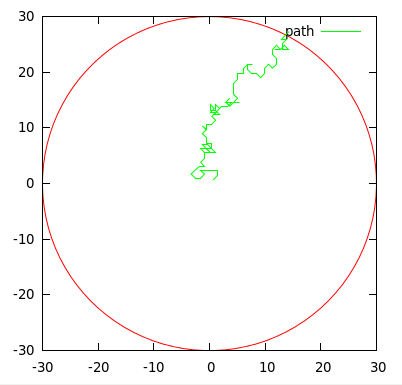
\includegraphics[width=0.49\textwidth]{r30_1.png}
	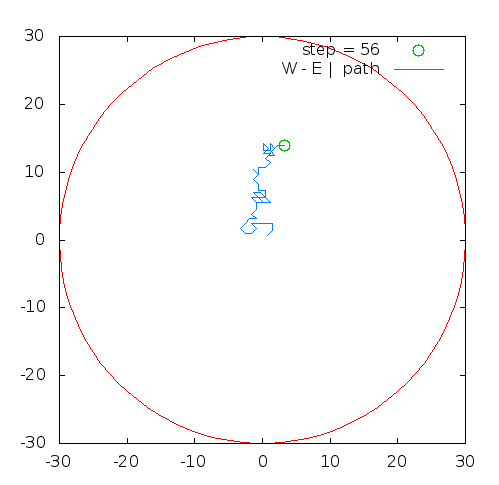
\includegraphics[width=0.49\textwidth]{r30_2.png}
	\caption{(kiri) Plot untuk batas $R_{max} = 30$, (kanan) cuplikan animasi.}
\end{figure}

\newpage
Untuk 1000 kali percobaan dengan $R_{max}$ berbeda,
\begin{figure}
	\centering
	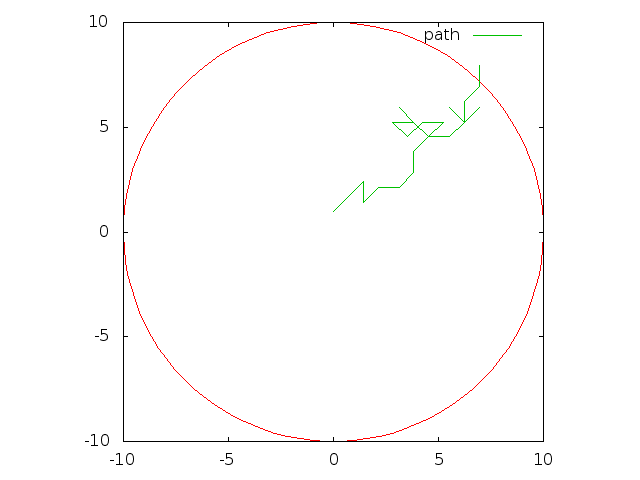
\includegraphics[width=0.24\textwidth]{hiker-plot-10-1.png}
	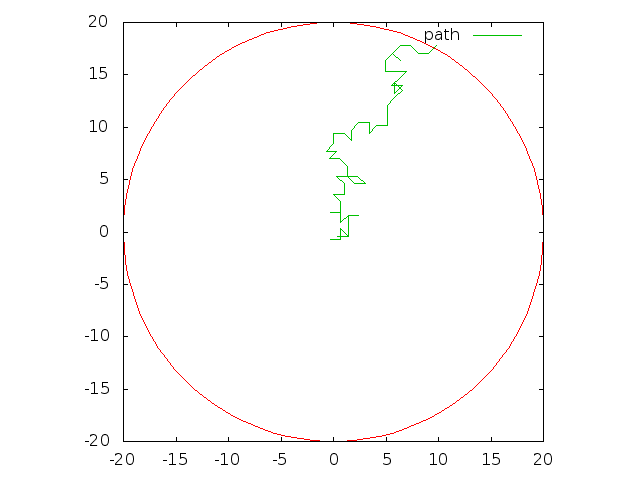
\includegraphics[width=0.24\textwidth]{hiker-plot-20-1.png}
	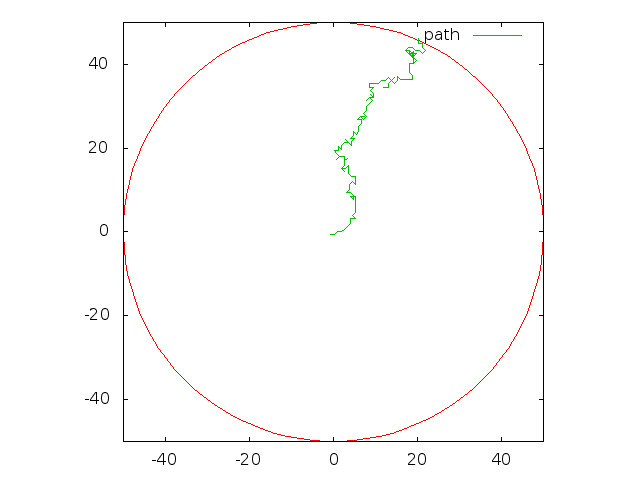
\includegraphics[width=0.24\textwidth]{hiker-plot-50-1.png}
	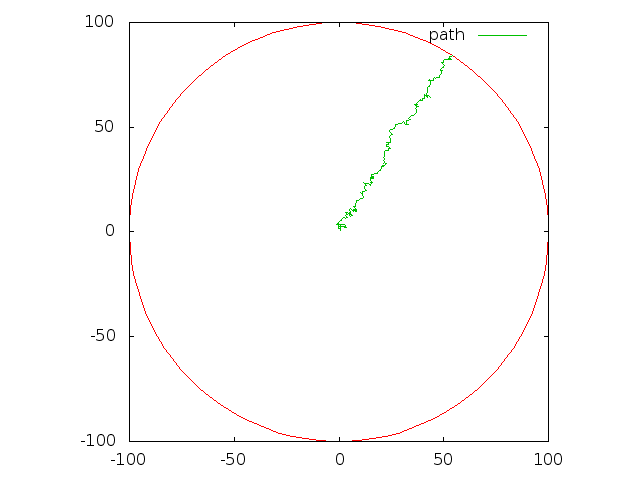
\includegraphics[width=0.24\textwidth]{hiker-plot-100-1.png}
	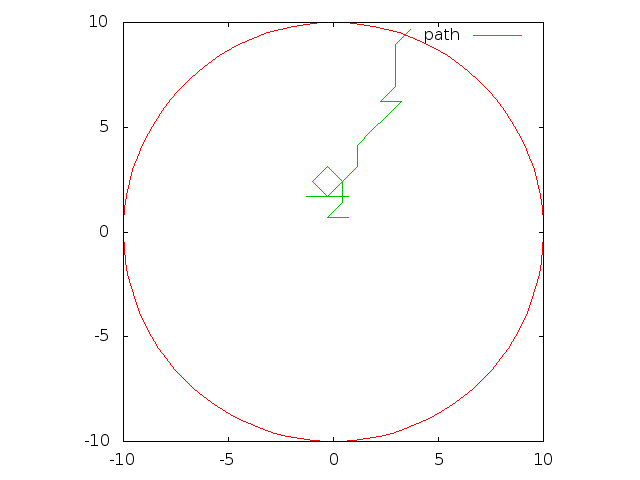
\includegraphics[width=0.24\textwidth]{hiker-plot-10-2.png}
	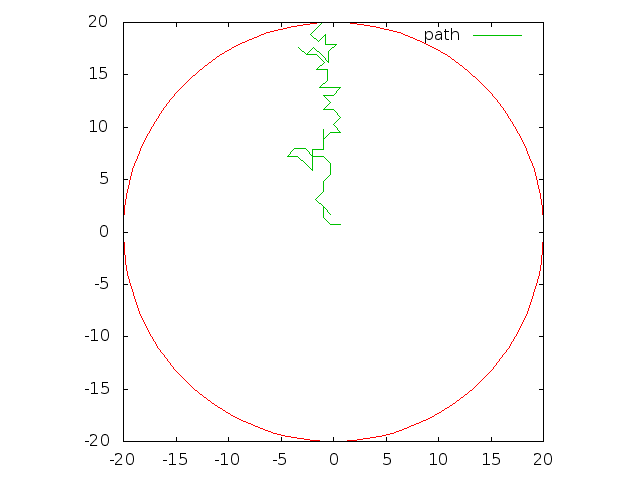
\includegraphics[width=0.24\textwidth]{hiker-plot-20-2.png}
	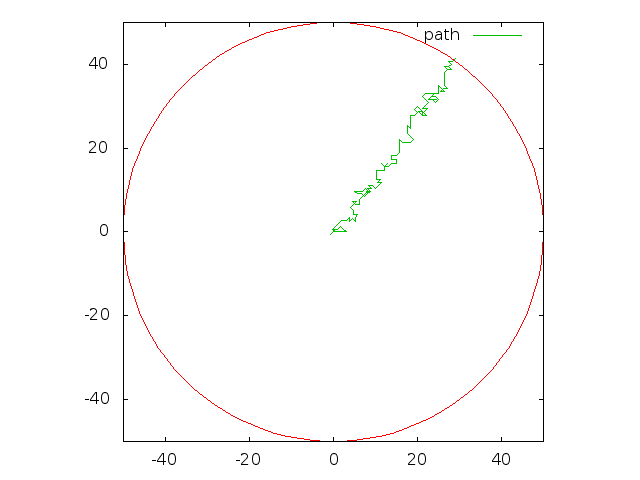
\includegraphics[width=0.24\textwidth]{hiker-plot-50-2.png}
	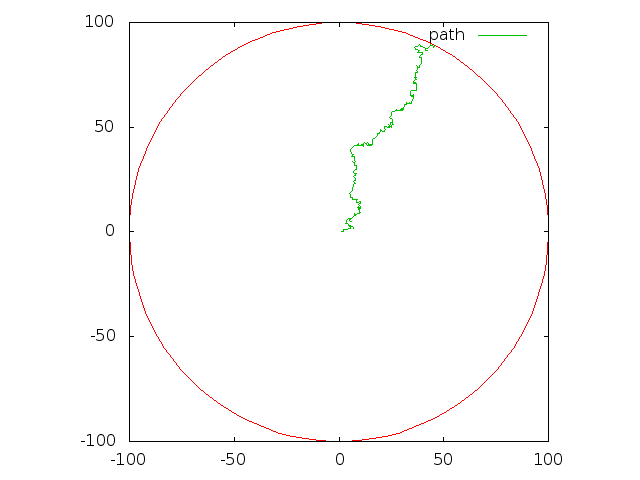
\includegraphics[width=0.24\textwidth]{hiker-plot-100-2.png}
	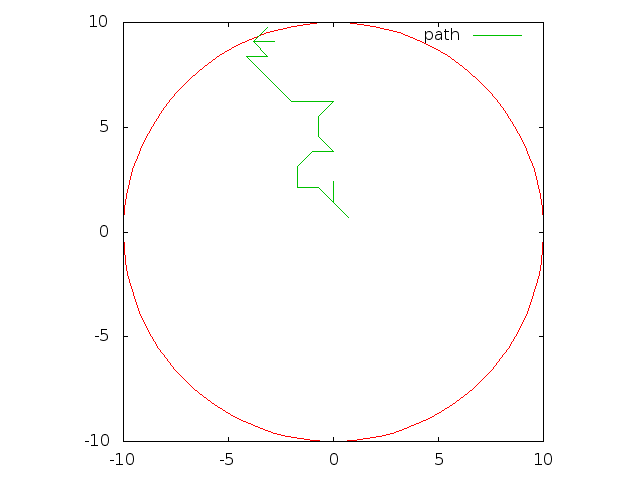
\includegraphics[width=0.24\textwidth]{hiker-plot-10-3.png}
	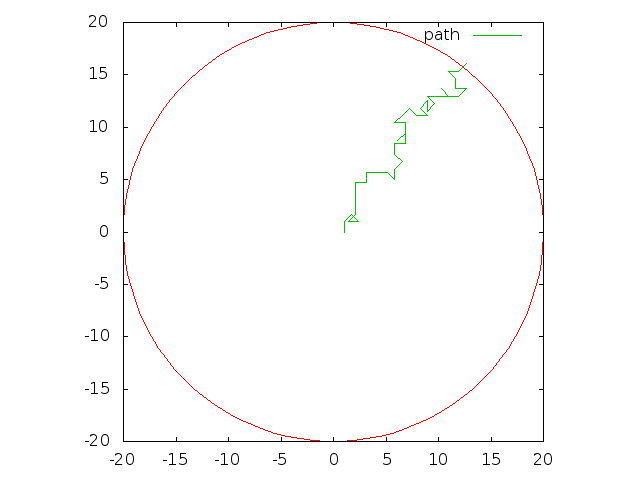
\includegraphics[width=0.24\textwidth]{hiker-plot-20-3.png}
	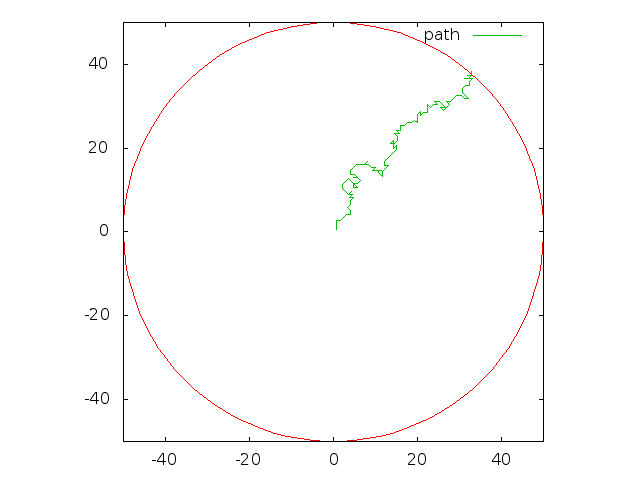
\includegraphics[width=0.24\textwidth]{hiker-plot-50-3.png}
	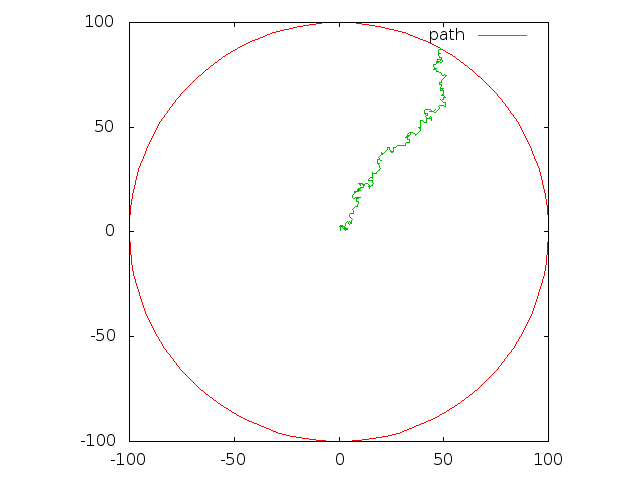
\includegraphics[width=0.24\textwidth]{hiker-plot-100-3.png}
	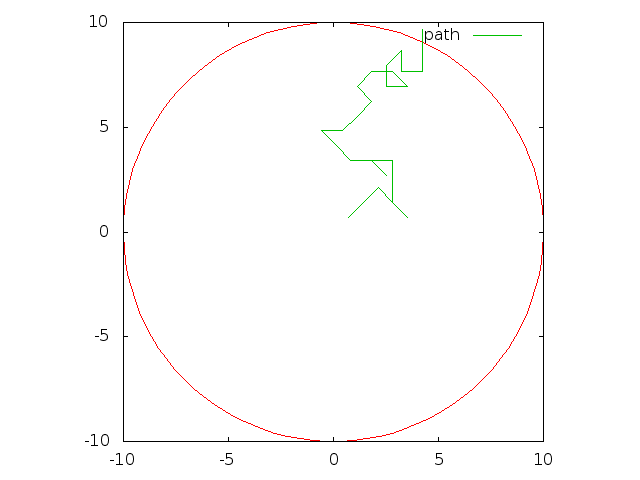
\includegraphics[width=0.24\textwidth]{hiker-plot-10-4.png}
	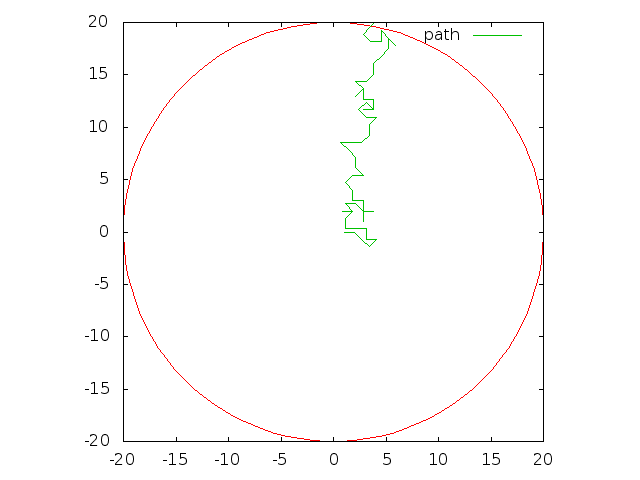
\includegraphics[width=0.24\textwidth]{hiker-plot-20-4.png}
	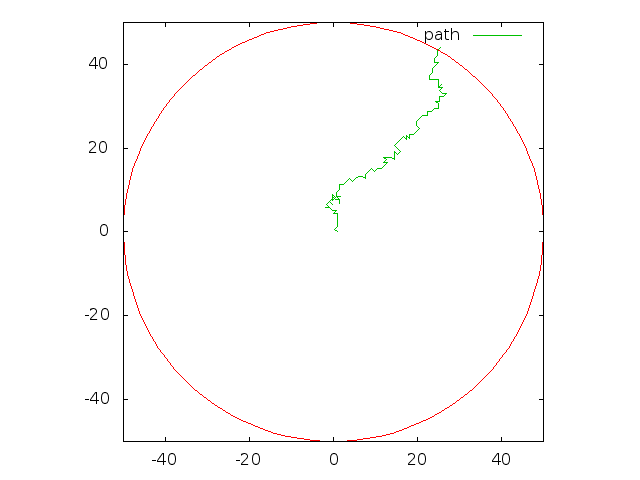
\includegraphics[width=0.24\textwidth]{hiker-plot-50-4.png}
	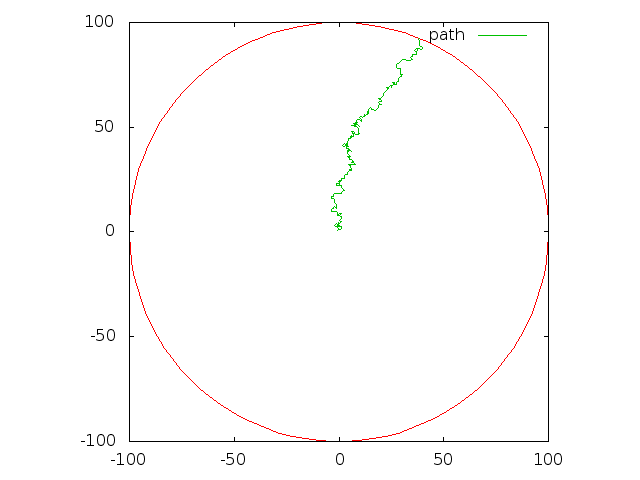
\includegraphics[width=0.24\textwidth]{hiker-plot-100-4.png}
	\caption{Contoh hasil run dengan $R_{max}$ yang berbeda. Urutan dari paling kiri, $R_{max} = 10, 20, 50, 100$.}
\end{figure}

Distribusi sudut posisi akhir (di $R_{max}$) terhadap posisi awal (1000 kali running):
\begin{figure}
	\centering
	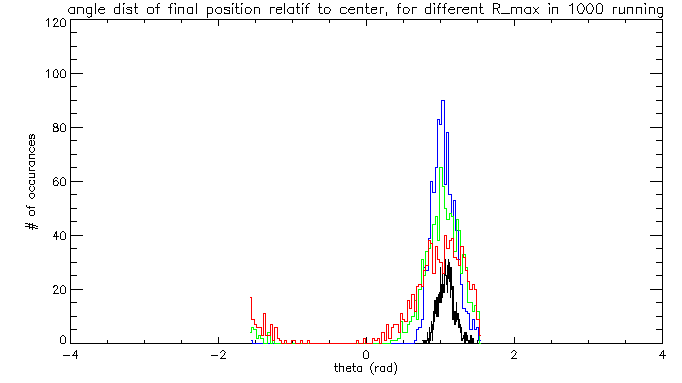
\includegraphics[width=0.65\textwidth]{hiker-theta.PNG}
	\caption{Merah untuk $R_{max} = 10$, Hijau untuk $R_{max} = 20$, Biru untuk $R_{max} = 50$, Hitam untuk $R_{max} = 100$.}
\end{figure}

\newpage
Distribusi jumlah step total (1000 kali running):
\begin{figure}
	\centering
	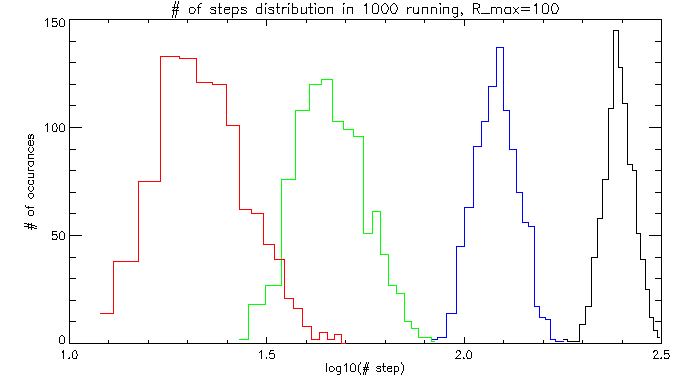
\includegraphics[width=0.7\textwidth]{hiker-nstep.PNG}
	\caption{Merah untuk $R_{max} = 10$, Hijau untuk $R_{max} = 20$, Biru untuk $R_{max} = 50$, Hitam untuk $R_{max} = 100$.}
\end{figure}

\textbf{Diskusi}
\begin{itemize}


\item dari distribusi posisi akhir (arahnya) untuk 1000 kali running diperlihatkan bahwa kecenderungan \textit{hiker} bergerak ke arah sekitar NE.
\item semakin lama hiker berjalan ($>R_{max}$) maka distribusinya semakin mengerucut ke arah sekitar NE. dan tidak ada pencilan ke arah sekitar N\---NW.
\item dari distribusi jumlah step, maka dapat dilihat untuk semakin jauh yang dituju ($>R_{max}$), dibutuhkan jumlah step \textit{randomwalk} lebih banyak, dan terkait secara \textit{power log} (dibutuhkan pemeriksaan lebih lanjut dan fitting).
\end{itemize}

\vspace{1.5cm}
\textit{\textbf{Brownian motion of pollen in the liquid}}\\
Simulasi yang sedikit lebih mendekati kasus sebenarnya dapat dilakukan dengan cara membuat sejumlah partikel kecil sebagai molekul liquidnya dan partikel lain yang jauh lebih besar sebagai pollen. Kemudian dapat dibuat semuanya bergerak dan setiap waktu dicek interaksi tumbukan dari semua pertikel, dan setiap pertikel bertumbukan maka arah gerak dan kecepatannya berubah sesuai momentum awalnya (misal dibuat lenting sempurna).
Namun untuk penyederhanaan lagi, kami buat simulasi dengan menggunakan randomwalk 3D saja, namun dengan step yang random pula.\\
Simulasi randomwalk 100 pollen tanpa interkasi tersebut kami buat dengan C++ dan \textit{gnuplot}, dan juga C++ dengan \textit{OpenGL} (kode terlampir).\\

Cuplikan hasilnya sebagai berikut:
\begin{figure}
	\centering
	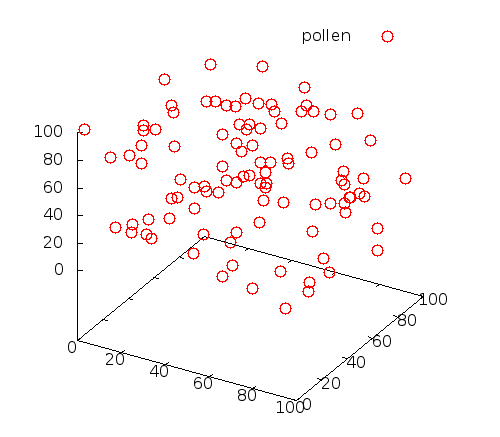
\includegraphics[width=0.45\textwidth]{pollen-gplt.png}
	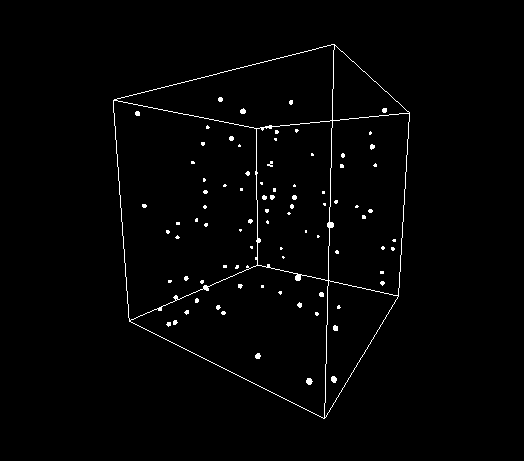
\includegraphics[width=0.45\textwidth]{pollen-ogl.png}
	\caption{Simulasi menggunakan \textit{gnuplot} (kiri), dan simulasi menggunakan \textit{OpenGL} (kanan).}
\end{figure}

Simulasi randomwalk tersebut menggunakan koordinat bola untuk menentukan arah geraknya, sehingga fungsi randomnya perlu dicek terlebih dahulu. Untuk membuat arah random yang benar fungsinya dibuat sebagai berikut:\\
$ \phi = 2 \pi r_{1}$\\
$\theta = arccos(1 - 2 r_{2} )$\\
karena apabila $\theta$ kita buat hanya berupa random antara 1 dan $\pi$ maka hasilnya akan tidak random (menghasilkan data di kutub lebih banyak dibandingkan dengan di ekuatornya). Hasil cek yang dilakukan sebagai berikut:
\begin{figure}
	\centering
	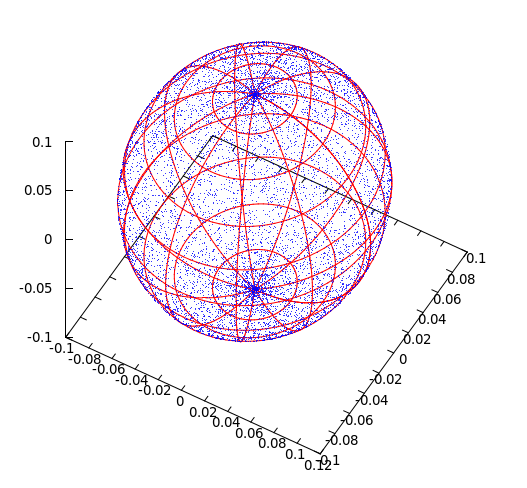
\includegraphics[width=0.45\textwidth]{distribusibola-salah.png}
	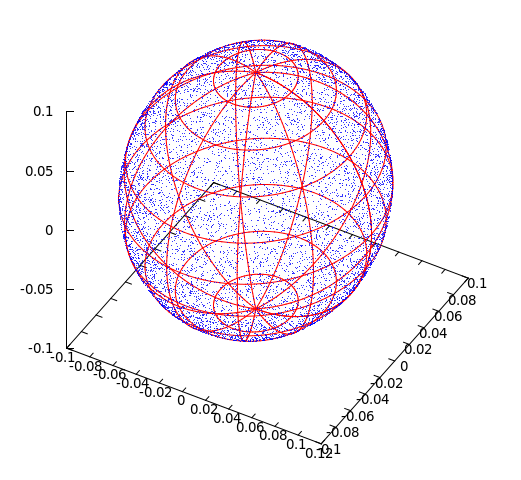
\includegraphics[width=0.45\textwidth]{distribusibola-benar.png}
	\caption{random salah (kiri), random benar (kanan).}
\end{figure}


\newpage
\textbf{LAMPIRAN}\\
\textit{Kode untuk gnuplot}
\lstset{frameround=fttt}
\begin{lstlisting}
// Copyleft (c) 2012. Ridlo W. Wibowo
// pollen.cpp
#include<iostream>
#include<stdlib.h>
#include<stdio.h>
#include<math.h>
#include<time.h>
#include<fstream>
#define _USE_MATH_DEFINES
using namespace std;

double phi, theta, l;
double unirand(){ return (double)rand()/(double)RAND_MAX;}

int main(){
    int n=100;
    double x[100], y[100], z[100];
    double dx, dy, dz;
    double xm=100., ym=100., zm=100.;
    int t = 0, tf=1000;

    srand(time(NULL));
    // inisiasi
    ofstream out("pollen-out.txt");
    for (int i=0;i<n;i++){
        x[i] = xm*unirand();
        y[i] = ym*unirand();
        z[i] = zm*unirand();
        out << x[i] << " " << y[i] << " " << z[i] << endl;
    }

    do{
	out << "\n\n";
        for (int i=0;i<n;i++){
            phi = 2.*M_PI*unirand();
            theta = acos(1. - 2.*unirand());
            l = unirand();
            dx = l*sin(theta)*cos(phi);
            dy = l*sin(theta)*sin(phi);
            dz = l*cos(theta);
            
            x[i] = fmod((x[i] + dx + xm),xm); // periodic boundary (toroida)
            y[i] = fmod((y[i] + dy + ym),ym);
            z[i] = fmod((z[i] + dz + zm),zm);
            
            out << x[i] << " " << y[i] << " " << z[i] << endl;
            }
         
         t = t+1;
    } while(t < tf);
    out.close();

    return 0;
}
\end{lstlisting}

\vspace{2cm}
\textit{\textit{Kode untuk OpenGL}}
\lstset{frameround=fttt}
\begin{lstlisting}
/**************************************************/
/* pollen.cpp                                     */
/* copyleft (c) 2012. Ridlo W. Wibowo             */
/**************************************************/
#include<GL/gl.h>
#include<GL/glu.h>
#include<GL/glut.h>
#include<iostream>
#include<stdlib.h>
#include<math.h>
#include<time.h>

int n=100;
double x[100], y[100], z[100];
double dx, dy, dz;
double l, theta, phi;
double unirand(){ return (double)rand()/(double)RAND_MAX;}

void init(void){
    glClearColor(0.0, 0.0, 0.0, 0.0);
    glShadeModel(GL_FLAT);
}

void move(){
    for (int i=0;i<n;i++){
        phi = 2.*M_PI*unirand();
        theta = acos(1. - 2.*unirand());
        l = 0.05*unirand();
        dx = l*sin(theta)*cos(phi);
        dy = l*sin(theta)*sin(phi);
        dz = l*cos(theta);
        
        x[i] = fmod((x[i] + dx + 5.),5.); // periodic boundary (toroida)
        y[i] = fmod((y[i] + dy + 5.),5.);
        z[i] = fmod((z[i] + dz + 5.),5.);
    }
}

void myIdleFunc(int a) {
    move();
    glutPostRedisplay();
    glutTimerFunc(100, myIdleFunc, 0);
}


void display(void){
    glClear(GL_COLOR_BUFFER_BIT);
    glColor3f (1.0, 1.0, 1.0);
    
    glutWireCube(5.0);
    for (int i=0;i<n;i++){
        glPushMatrix();
        glTranslatef(-2.5 + x[i], -2.5 + y[i], -2.5 + z[i]);
        glutSolidSphere(0.05, 10, 8);
        glPopMatrix();
    }
    glutSwapBuffers();
}

void inisiasi(){
    for (int i=0;i<n;i++){
        x[i] = 5.*unirand();
        y[i] = 5.*unirand();
        z[i] = 5.*unirand();
    }
}


void reshape(int w, int h){
    glViewport(0, 0, (GLsizei) w, (GLsizei) h);
    glMatrixMode (GL_PROJECTION);
    glLoadIdentity();
    gluPerspective(100.0, (GLfloat) w/ (GLfloat) h, 1.0, 20.0);
    glMatrixMode(GL_MODELVIEW);
    glLoadIdentity();
    gluLookAt(4.0, 1.0, 6.0, 0.0, 0.0, 0.0, 0.0, 1.0, 0.0);
}

int main(int argc, char** argv){
    glutInit(&argc, argv);
    glutInitDisplayMode(GLUT_DOUBLE | GLUT_RGB);
    glutInitWindowSize (700, 700);
    glutInitWindowPosition (100, 100);
    glutCreateWindow ("pollen brownian motion");
    init ();
    srand(time(NULL));
    inisiasi();
    glutReshapeFunc(reshape);
    glutDisplayFunc(display);
    glutTimerFunc(100, myIdleFunc, 0);

    glutMainLoop();
    return 0;
}
\end{lstlisting}

Simulasi kami upload di \url{http://astrokode.wordpress.com/}

\end{document}
